\documentclass{report}

\usepackage[margin=1.5in]{geometry}

\usepackage{float}
\usepackage{graphicx}
\usepackage{hyperref}
\hypersetup{colorlinks=true,linkcolor=blue}
\usepackage{pdfpages}

\usepackage{listings}
\lstMakeShortInline{|}
\lstset{columns=flexible,language=SQL,basicstyle=\ttfamily}

\def\sectionautorefname{Section}
\def\subsectionautorefname{Section}
\def\subsubsectionautorefname{Section}

\newcommand{\myref}[1]{\autoref{#1} on page \pageref*{#1}}
\newcommand{\tabref}[1]{\lstinline|#1| table (see \myref{tab:#1})}

\newcommand{\intern}{This table may be interned, see \myref{def:intern}.}

\setlength{\belowcaptionskip}{10pt}

\begin{document}

\begin{titlepage}
  \begin{center}
    
\includegraphics[width=10cm]{../../lib/images/bluej-icon-256.png}\\
    \huge BlueJ Blackbox Data Collection\\~\\Researchers' Handbook
    (version 1.7, ? July 2017)
  \end{center}
\end{titlepage}

\section*{Getting Started}

This document acts as a manual for the BlueJ data collection project,
``Blackbox''.  It is intended to explain, in detail, the schema of the
collected data, and how the data relates to the BlueJ IDE.  It assumes a basic
familiarity with BlueJ's capabilities, such as the debugger, codepad, object
bench and so on.

Chapter \ref{sec:concepts} explains the concepts, assumptions and caveats
associated with the data recording.  It is important to read this chapter
before carrying out any detailed analysis, so that you do not proceed with
false assumptions.  Chapters \ref{sec:master_events} and
\ref{sec:other_tables} contain technical detail on the data schema.

Chapter \ref{sec:data_access} contains details on how to actually access the
data (MySQL details, etc), and chapter \ref{sec:data_use} contains the
data-use policies which we expect all researchers to read.  Finally, chapter
\ref{sec:example_codeview} has details on the example application we have
provided, and chapter \ref{sec:postprocess} has some details on
post-processing we have in place.

\begingroup
\let\clearpage\relax
\tableofcontents
\endgroup

\listoftables

\begin{table}
\caption[Possible \lstinline!master_events.name! values]{List of different
  values allowed for the \lstinline!name! column in the \lstinline!master_events! column, with
  links to sections in which that event is described.}
\label{tab:event_names}
\begin{center}
%table:event_names
\end{center}
\end{table}

\chapter{Concepts and Caveats}
\label{sec:concepts}

There are several concepts involved in the Blackbox project, and it is
very important when doing analysis on the data to understand the concepts
involved, and particularly the limitations of the data collection.  If you
naively assume that one virtual user is one real person, you may draw false
conclusions from your analysis.

\section{Users}
\label{def:users}

BlueJ stores its properties file in a per-user location.  For example, on
Linux, it uses |~/.bluej/bluej.properties|, whereas on Windows 7 it is (on a typical
home installation) |C:\Users\Joe\bluej\bluej.properties|.

This properties file is the only mechanism that BlueJ has to have any sense of
identity.  If two physical people use the same account, they will appear to
BlueJ as a single user (this is still quite common on home Windows systems).
If someone uses BlueJ on a university machine, and on a laptop, and on a home
machine, they will appear to be three users.
If the computer is set up to not maintain a user's profile correctly (e.g. a
school system which wipes a user's profile on logout -- we know some systems
do this!), they will get a new profile each time they load BlueJ, and thus
will always appear to be a new user.  If the same bluej.properties file is
shared between many physical users (e.g. they all get the same profile on
login), they will all appear to be the same user (operating with many parallel sessions).

The user's unique identifier or opt-out preference is stored in this
properties file.  Thus the concept of a ``user'' is tied to the properties
file.  It is important to understand this when reasoning about users.

\section{Projects}
\label{def:projects}

BlueJ deals with projects.  A project is a directory with a BlueJ project
file, and source files (and class files, and maybe a README, and whatever else
the user stores in the directory).  In Blackbox terms, projects are associated
with particular user ids.  They are identified only by the associated user,
and their full path (hashed, for anonymity).

If a user makes a copy of a project and opens it, it will appear to be an
entirely separate project (though you could post-process the data to see that
the project has the same source code as another of the user's projects).  If a
user has the project on a USB memory stick, and it gets assigned a different
drive letter next time they plug the stick in, the project will appear to be
different.  If a person loads the project from two different machines, even if
the project has the same path on both machines, they will appear as separate
projects belonging to separate users.

\section{Packages}
\label{def:packages}

A project will have at least one package (the unnamed, default Java package),
and potentially many.  BlueJ displays a main interface window for each package
that the user opens within the project.  Thus there can be as many codepads as
there are packages in the project.  Some BlueJ features are per-package (codepad,
object bench), while others are per-project (debugger, version control).

\section{Sessions}
\label{def:sequence_id}

Each time that BlueJ is opened, we deem the time from the opening to the
closing to be ``a session''.  Each time BlueJ is loaded, the client generates
a unique session identifier to label all events from that session with.

If a user loads many projects at once in a single instance of BlueJ, these
will all count as one session.  If a user loads BlueJ twice in parallel
(e.g. by clicking the shortcut too many times), both sessions will be
recorded.  But for this reason, it is usually a good idea to use sessions and projects to
process events, rather than solely relying on event timestamps (which will
interleave events from the two sessions).  If a user accidentally closes BlueJ
and immediately re-opens it, that will count as two sessions (though you could
spot this using the timestamps on the events in post-processing).

There is no time limit on how long a session can last -- the client-generated
identifier is relied upon to differentiate sessions.  It is possible for a
session to last for weeks if a user keeps BlueJ open on their always-on
machine.  One potentially common case is that if a user never shuts down their
laptop, and instead always makes it sleep, the session can last for a long
time if they leave BlueJ open on their laptop (but see
\myref{def:interruption} for why they may not send us much data this way, if the session
stops sending data at any point).

\section{Participants}
\label{sec:participants}

All the data in the BlueJ data collection is anonymous.  Part of the intention
of the project is to support local experiments, where you, the local
researchers, collect additional information about users.  The additional
information should be held by you, and the experiment approved and conducted
according to your local ethics committee.

To allow you to link your participant data with our data, we have a mechanism
for BlueJ users to specify an experiment identifier and a participant
identifier (strings, up to 32 characters).  These two identifiers should be
assigned by you, the local researcher.  We request that you assign an
experiment identifier that is unlikely to clash with other researcher's
identifiers.  The participant identifier is entirely up to you, although we
would expect that you use a generic identifier (e.g. a number), and that you
hold the mapping between the participant's real identity and the participant
number, as is standard practice.  (That is: do not ask the participants to store their name, or
university login or similar, in the participant identifier.)

As described in section \myref{sec:views}, you will be able to retrieve
participant identifiers for a specific experiment identifier, and retrieve
session data for known experiment identifiers and participant identifiers.
This means that you will not be able to see experiment or participant
identifiers for experiments for which you do  not know the identifier.  This
is deliberate, to help protect information about experiment participation and
participant identification.

\section{Events}

The BlueJ client sends a stream of events to the BlueJ server, which
acknowledges them.  Ultimately, all the information recorded on the server
came by way of these discrete events.  Things like users or sessions are
reconstructed from the individual events that have been sent.  Every event
that the server receives, without exception, is recorded with an entry in the \tabref{master_events}.

\section{Interrupted Connections}
\label{def:interruption}

There are potential problems with missing events or entire sessions in the
event stream for a user.  You should
never assume you have a user's complete history of interaction with BlueJ.
Notably, entire sessions might be missing due to users using BlueJ without an
internet connection (e.g. on an aeroplane).  Similarly, you should not assume
that you can see all interactions with a project -- source code could be
edited outside BlueJ.

Within a session, you can assume that you have all events, sequentially
consistent, from the first \texttt{bluej\_start} event, up until the last
event that is recorded in the session.  This may not be the actual final event
that the user performed in their real session -- the user's
internet connection may drop, or BlueJ may crash or get killed before a batch of events
is sent, and so on.  But there will never be a ``hole'' in the middle of a
session where events are lost, then resumed again.  \textbf{Any event that fails to
send will cause the BlueJ client to stop sending for the rest of the session}
-- each event is only sent once the event before it in the session has succeeded.

It is a deliberate decision to not attempt to resume sending data if previous
data has failed to send.  Part of this decision is technical -- we do not want
to keep retrying a send if the user has no Internet connection (or if our own
server is inaccessible for some reason), and we do not want to cache lots of
events on the client in the hope that the connection one day re-appears.

The other reason is that analysis becomes much harder if events within a session
may be missing -- data consistency is a nightmare.  For example, you may see
that a user has closed an inspector, but not how that inspector appeared.  Or
you may see an execution take place, but not know what breakpoints are set in
the code.  If gaps are allowed in the event stream, we would have to send a
lot more state information with each event to make analysis possible.

\section{Spam}
\label{def:spam}

The BlueJ data collection project server is an open web server to which anyone
can submit, and the BlueJ client is an open-source program.  There is no
technical way to guarantee that the data coming in is from an unmodified BlueJ
client -- it could be modified, or it could simply be made-up spam data being
submitted.  It remains to be seen whether this will be an issue.

\section{Source Code Consistency}

When a package is opened, the full state of the source code of the project is
sent to the server.  Similarly, when a class is added to the project while
BlueJ is running, the full code is sent.  For all other edit events within a session, a diff is sent
between the last successfully sent source code state (during that session) and
the new state.  Using a diff minimises the amount of data sent and stored.

You can assume that the source code diffs within a session are consistent.
However, you should not assume that you have seen the full state of the source
code between sessions.  Source code may be edited outside BlueJ or may be edited
by BlueJ when the user has no Internet connection.  You should be able to
detect this by comparing the source code state between the end of one session
and the start of the next.

\section{The Debug VM}

BlueJ has two virtual machines.  One, generally known as the server VM,
handles:

\begin{itemize}
\item The graphical interface
\item Code editing
\item Compilation
\end{itemize}

No user code is ever run on the server VM.  All user code is run on a second
VM, known as the client VM or the debug VM.  (There is only ever one debug VM
at a time, for each project.)  So things like:

\begin{itemize}
\item Object construction
\item Method invocations
\item Codepad use
\item JUnit tests
\end{itemize}

Are all run on the debug VM.  When the debugger is used, the interface and
control code are in the server VM, using hooks into the debug VM to do
stepping and so on.  Whenever user code is executed, it is possible that the
result is that the debug VM terminates, but this does not mean that BlueJ has
exited.  User code that runs forever will not interrupt BlueJ, but will
prevent further use of the debug VM.


\section{Extensions}

BlueJ has an extension mechanism that allows programmatic operation of BlueJ
from third-party extensions.  (Not to mention that BlueJ is open-source,
anyway.)  The extensions can trigger many of the events described in this
document.  We do not annotate which events are triggered by extensions and
which are not.  This annotation would be a lot of extra technical work, and
probably for not much purpose, since we do not believe many BlueJ users use
extensions that will trigger these events.

We do record which extensions are loaded in the blackbox data, so you can use
this to rule out any extensions which could be problematic (or more likely, to
whitelist extensions that are not an issue).


\section{Database Structure and Notes}
\label{sec:assoc}

The database is used as a persistence layer by our Ruby on Rails server, which
uses an object-store model.  Every table in the database, except many-to-many link tables, has an
integer |id| field which acts as a primary key.  Relations in the database are
handled in two ways:

\begin{enumerate}
\item When the destination table is fixed and known -- e.g. a master event has a user --
  there is a field in the |master_events| table named |user_id| which links to
  the |users| table.
\item When the destination table may vary, e.g. a master event has a subordinate
  ``event'' record which may be from one of many tables, there is both an
  |event_id| and an |event_type| field.  The |event_type| field contains an
  uppercased camel-cased, non-underscored\footnote{This is Rails' doing -- don't ask.} version
  of the table name.  So if a particular master event links to a compile
  event, the |event_type| field will have |"CompileEvent"|, and the |event_id|
  will correspond to an |id| in the |compile_events| table.
\end{enumerate}

\subsection{Interning}
\label{def:intern}

There are some tables in the database which are likely to feature the same
information over and over again, such as the installation details.  When the
server comes to add a record to these tables with duplicate data to a previous
record, it \textit{may} reference the existing record instead, to save space, like
interning strings.  This is a performance optimisation that should have no
effect on the semantics.  Tables that do this are tagged as such.

\chapter{Master Events Table}
\label{sec:master_events}

The master events table is the place where all events are entered.  There are
lots of different types of events that can be received, each with a variety of
different data, but all of them get one entry in the |master_events|
table, with links to other tables where necessary.

%schema:master_events

The most important field in the table is the |name| field, which describes
which kind of event it is, and determines which of the other fields will be
present.  The possible values for the |name| field are given in \myref{tab:event_names}.

Each master event has links (as per \myref{sec:assoc}) to other tables:
\begin{itemize}
\item |user_id| -- present for all events
\item |session_id| -- present for all events
\item |project_id| -- present for all events except |"bluej_start"| and |"bluej_finish"|
\item |package_id| -- present for some events (see further details below).
\item |event_id|, |event_type| -- present for some events (see further details below).
\item |participant_id| -- present for all events, if the user currently has
  participant information specified.
\item |client_address_id| -- present for all events.
\end{itemize}

The |created_at| field is a server-side, trustworthy datestamp of when
the event was received.  The |source_time| is the client-side time,
which is likely (but not guaranteed) to be sequentially consistent, but should
not be trusted to be accurate.

The |sequence_num| field is provided by the client to make sure events are
received in correct sequence (within a given session).  The server ensures
that the sequence numbers are valid (i.e. that they begin at 1, and each
subsequent event increments the sequence number by 1).

%hidden:participants

The |participant_id| field links to a hidden |participants| table.  If you
want to investigate this information, see \myref{sec:views} on how to
access this information.

%hidden:client_addresses

The |client_address_id| field links to a hidden |client_address| table.  Details
on using |client_address_id| to get at user locations are given in \myref{sec:locations}.


The subsequent sections in this chapter describe the different possible values for the
|master_events.name| field, and what that means for the other fields,
especially what is linked to by the |event_id| and |event_type| fields.  Each
section title has a string, which is the value of the |name| field.

\section{Start/Finish Events}

Two bookend events are sent, one when BlueJ starts (before it has loaded up a
project or done anything) and one when BlueJ exits (after it has closed all
projects and finished everything).  The data will likely contain more start
events than finish events, for reasons explained in \myref{def:interruption}.

\subsection{\lstinline!"bluej_start"! and \lstinline!"bluej_finish"!}

These two events have no extra accompanying event.  They have no |project_id|
and no |package_id|.  However, the |"bluej_start"| event will have zero or more
attached entries in the \tabref{extensions} that link back to this master
event -- these are extensions loaded from the system directories.

The |"bluej_start"| event will always create a new entry in the
\tabref{sessions} -- the installation details for this copy of BlueJ will be
recorded there.

\section{Project Events}

When a project is opened or closed in BlueJ, corresponding events will be
sent.  See \myref{def:projects} for details on how projects are
distinguished.  A project-open event will be followed by at least one
package-open event.

\subsection{\lstinline!"project_opening"!}

This event has no |package_id|.

This event will have zero or more entries in the \tabref{extensions} linking
back to this event, which represent extensions loaded from this project's directory.

\subsection{\lstinline!"project_closing"!}

This event will no attached data, and will have no |package_id|.

\section{Package Events}

When a package is opened or closed in BlueJ, a corresponding event is
generated.  Note that each window in BlueJ actually belongs to a package.

\subsection{\lstinline!"package_opening"!}

This event will have a |package_id|.

The event will have zero or more entries in the \tabref{source_histories} that
link back to this event.  These represent the state of the files as the project is
opened (as a |complete| snapshot, not a diff).

The event will link to an entry in the |source_hashes| table
(|event_type| will be |"SourceHash"|), which will contain a hash of
the source code in the package.  The exact details of the hash are
unimportant, but this hash can be used to quickly narrow down likely
duplicate projects (for example, spotting the starting projects from
the BlueJ book).

%schema:source_hashes \intern

\subsection{\lstinline!"package_closing"!}

This event will have a |package_id|.  For BlueJ 3.x, there is no associated
event or associated source histories.

For BlueJ 4.x, the event will have zero or more entries in the \tabref{source_histories} that
link back to this event.  These represent the state of the files as the project is
opened (as a |complete| snapshot, not a diff).

For BlueJ 4.x, the event will link to an entry in the |source_hashes| table
(|event_type| will be |"SourceHash"|), which will contain a hash of
the source code in the package.  Such a hash uses the same hashing algorithm
as the |"package_opening"| event.


\section{Editing}

We do not capture all the different edit operations (e.g. paste, indent), we
only capture the resulting effect on the source code.

\subsection{\lstinline!"edit"!}

This event will have a |package_id|, pointing to the package of the class that
is edited.

This event is the central editing event in BlueJ.  These events are recorded
when multiple lines are edited at once (e.g. via paste, or deleting a
selection, or so on), or a single line has been edited and the caret
has now left that edited line.  An edit event is not generated by every single
keystroke.

There is currently no guarantee as to how edits are grouped together into a single edit
event (e.g. highlighting a selection and then pasting may appear as one event
or two events, auto-indent may appear as one edit or several edits, and many
other such examples), but an edit event will never span a compiler event, and
all edits will be flushed before a compile event.

If a Java file was edited, the event will always have exactly one associated entry in the
\tabref{source_histories}, which will be a |"diff"| event.  If a Stride file was edited,
the event will have two associated entries \tabref{source_histories}, which will be a |"diff"| event
for the Stride file and a |"diff_generated"| event for the generated Java file.

\subsection{\lstinline!"file_add"!}

This event will have a |package_id|, which indicates which package the file
was added to.

This event is fired whenever a class is added to the BlueJ project.  This may
be via the New Class menu item, or via the Import Class menu item, or via
version control.

The event will always have either one or two associated entry in the
\tabref{source_histories}, which will be a |"complete"| event.  One, if this
is Java file.  Two, if this is a Stride file (one for the Stride file, one
for the generated Java file).

\subsection{\lstinline!"file_delete"!}

This event will have a |package_id|, which indicates which package the file
was deleted from.

This event is fired whenever a class is removed from a BlueJ project.  This
may be via the interface, or via version control.

The event will always have exactly one associated entry in the
\tabref{source_histories}, which will be a |"file_delete"| event.

\subsection{\lstinline!"rename"!}

This event will have a |package_id|, which indicates which package the file
was renamed in.

This event is fired whenever a class is renamed in a BlueJ project.  A rename
occurs in BlueJ when a Java file is saved, and is parseable, and has a
different top-level class name to the name of the file.  At this point, BlueJ
silently renames the file to match the class name.  But note that until this
save occurs, many more edits may take place, so the rename of the file may
appear some time after the actual relevant source code edit takes place.

The event will always have exactly one associated entry in the
\tabref{source_histories}, which will be a |rename| event.

\subsection{\lstinline!"convert_stride_to_java"! (since BlueJ 4.x)}

This event will have a |package_id|, which indicates which package the file
was renamed in.

This event is fired when the user permanently converts a Stride class to Java.

The event will always have two associated entries in the
\tabref{source_histories}.  One entry will be a |stride_to_java| event, which will
be associated with the Java source file (i.e. the \textit{target} of the conversion).  The content
  of this event will be a diff against the previous state of the Java file, as in a diff event.  Note that the Java file exists before and after the conversion, but switches from being auto-generated to being user-edited.
The other source history entry will be a |file_delete| event, which will be associated with the Stride file (since it gets
removed as part of the conversion).

\subsection{\lstinline!"convert_java_to_stride"! (since BlueJ 4.x)}

This event will have a |package_id|, which indicates which package the file
was renamed in.

This event is fired when the user permanently converts a Java class to Stride.

The event will always have two associated entries in the
\tabref{source_histories}.  One entry will be a |java_to_stride| event, which will
be associated with the Stride source file (i.e. the \textit{target} of the conversion).  The content
  of this event will the complete content of the new Stride file, as in a file creation event.
The other source history entry will be a |java_gen_from_stride| event, which will be associated with the Java file, and contains a diff from the previous state of the Java file.  Note that the Java file exists before and after the conversion, but switches from being user-edited to being auto-generated.

\subsection{\lstinline!"file_open"!, \lstinline!"file_select"! and \lstinline!"file_close"!}

This event will have a |package_id|, which indicates which package the relevant file
was in.

These three events will only be recorded in versions of BlueJ from 4.0.0 onwards, and
in Greenfoot.

These three events do not affect the content of a file, but instead correspond to
GUI actions: opening a source file for editing, focusing the editor of a source file, and
closing a source file.  A select or close should always be preceded in a session by an
open event for the file, and an open event is typically immediately followed by a
select event (but this may not always be the case, if the editor opens in the background).
It should not be possible for two open events to occur for a file without a close event
inbetween, but don't take that as a cast-iron guarantee.

A select event occurs when the user switches tab in an already-focused tabbed editor window,
and for the current tab when the editor window receives the focus.

A close event occurs when the tab is closed, either individually or because the tabbed editor
window was closed.  It may be possible for a BlueJ session to finish without all editors being
closed first.

Each event will always have exactly one associated entry in the \tabref{source_files},
indicating the relevant file.

\section{Compilation}

Compilation is a core part of BlueJ and of the Blackbox data set.  There are differences in how
compilation works between Java-in-BlueJ-3.x, Java-in-BlueJ-4.x and Stride (which only exists in BlueJ 4.x),
but they all use the same database tables, with slightly different combinations of fields.

In BlueJ 3.x, Java compilation works as follows:

\begin{itemize}
\item The user can make any edits to their code without triggering compilation.
\item Compilation will only occur when the user requests it, or in a couple of other
uncommon situations, such as when an extension triggers compilation.
\item After compilation has finished, the first error (and only the first error) is
shown by highlighting the background of the line in red, and showing the error message
in the message pane at the bottom of the editor window.  We record which error was shown.
\end{itemize}

In BlueJ 4.x, Java compilation works as follows:
\begin{itemize}
\item While the user is editing, if their cursor leaves a line of code which has been
modified, we perform an ``automatic error check''.  We use this description to
distinguish the automatic error check (which just shows
errors, if any) from a compilation (which outputs new .class files if successful) in
the user's mind.  In reality, both feed the users' code into the Java compiler, and the
only difference is whether the class files are discarded (error check) or retained (compile)
if the internal compile is successful.
\item In Blackbox, both the automatic error check compilations and standard compilations
 are stored in the same compilation events table (as described later).
 Crucially, the new |compile_events.reason| field will let you distinguish between
 the different types.
\item After either error check or manual compile has finished, if there are errors then
all the errors are indicated on screen using a red underline.  For this reason, all
errors are marked as shown, meaning the indicator was shown.  There is a new separate
mechanism for recording when the actual error message was shown to the user.
\end{itemize}

In Stride, compilation works as follows:
\begin{itemize}
\item Once the user makes an edit, then we keep track, and as soon as they stop editing
for a period of time (currently 1 second), we perform an automatic error check (as per
Java in BlueJ 4.x).
\item Stride has an extra mechanism for deciding when to show error indicators.  Stride
has the notion of a ``fresh'' frame.  Essentially, we do not want to show errors in a frame
that the user has not yet finished.  So if the user is editing a new assignment frame, we do
not want to show an error about an empty right-hand side if they are still filling in the
 left-hand side.  So we count any newly-created frame as fresh, and no red error underlines
 are shown in fresh frames.  Hence any errors from an automatic error check are not shown for
 fresh frames, and will not be marked as shown.  If the user moves the focus out of that frame,
 the error indicator will be shown and a shown error indicator event will be fired for each one.
\item As with Java, there is a separate event for recording when the actual error message
(not the error underline indicator) is actually shown to the user.
\item Stride also has the notion of quick-fixes (currently Stride only).  Each error may optionally
have quick fix suggestions, such as renaming a mis-spelled variable, or importing an unknown class.
These are recorded when they are shown to the user (they are shown with the compile error message), and if they are actually executed by the user.
\end{itemize}

\subsection{\lstinline!"compile"!}

This event will have a |package_id| if and only if all the compiled files were
in the same package.  However, having a |package_id| does not necessarily
indicate that the user asked for the whole package to be compiled.

This event occurs whenever a compilation of the user's classes is triggered.
(This does not include things like codepad interactions).

This master event will always have |event_type| set to |"CompileEvent"|, and
|event_id| will reference an entry in the \tabref{compile_events}.  (In turn,
that entry in the |compile_events| table, will be linked to by one or more
|compile_inputs| and zero or more |compile_outputs|, but see the
\tabref{compile_events} for more details.)

Note that compilation has undergone an overhaul in BlueJ 4.x.  In BlueJ 4.x onwards, compilation is performed
automatically in a number of different cases.  This is/will be documented in the new
reason column in the \tabref{compile_events}.

\subsection{\lstinline!"shown_error_indicator"! (since BlueJ 4.x)}

Since BlueJ 4.x, error display has changed.  Errors
are no longer shown one at a time in BlueJ in the bottom pane.  Instead, red underlines
throughout the code (in Java and Stride editors) indicate an error.  So when compilation
has finished, the user will see one red underline for each error located.  (Where error locations
overlap, only one is shown.)

All Java errors are initially marked as shown, but in the sense that the red underline is shown.
Stride errors are marked as not shown, but those that do get their red underlines shown will later (possibly near-instantly)
get a |"shown_error_indicator"| event recorded.  This does not mean that the user has been shown
the error message: that is recorded by the |"shown_error_message"| event, below.

The |sub_event_type| of |"shown_error_message"| events will be |"CompileOutput"| and the |sub_event_id|
will contain an |id| from an entry in the \tabref{compile_outputs}.

\subsection{\lstinline!"shown_error_message"! (since BlueJ 4.x)}

For BlueJ 4.x, a |"shown_error_message"| master event is generated when the user is
actually shown the text of the error message, by using keyboard or mouse focus to hover in
the location of the red underline.  Each error (which is stored in the \tabref{compile_outputs}, below)
will only get an |"shown_error_message"| event generated once, the first time it is shown.  If another
compilation occurs, an error with the same text at the same location will get a new entry in the
\tabref{compile_outputs}, and thus be considered a new error.  This all applies to Java and Stride.

The |sub_event_type| of |"shown_error_message"| events will be |"CompileOutput"| and the |sub_event_id|
will contain an |id| from an entry in the \tabref{compile_outputs}.

In Stride, when an error is shown, it may be presented along with a list of quick fixes (e.g.
correcting a typo in a variable name).  In this case, there will be entries recorded in the
\tabref{quick_fixes} table.  If one of these fixes is executed it will lead to a |"fix_executed"|
event being generated.

\subsection{\lstinline!"fix_executed"! (since BlueJ 4.x)}

As described in the previous section, a Stride error may be shown along with some suggested quick
fixes.  These are recorded in the \tabref{quick_fixes}.  If the user selects to execute one
of the quick fixes, a |"fix_executed"| master event is generated, where the |sub_event_type| is |"QuickFix"|
and the |sub_event_id| is the |id| of an item in the \tabref{quick_fixes}.

\subsection{Related Tables}

The |compile_events| table records whether the compilation was a success
(i.e. no errors -- but there could be warnings) or not.

%schema:compile_events

The |compile_events| may then be linked to by entries in the |compile_inputs| and
|compile_outputs| table.  The reason column was added in BlueJ 4.x.
Possible values for reason are:

\begin{itemize}
\item |NULL| -- This indicates the compile event occurred in BlueJ 3.x, which predates
the addition of the reason column.
\item |"early"| -- A check in Stride for errors that can be spotted without full javac
 compilation, such as a slot being empty or having a parse error.  Early compiles are only recorded if they feature errors.
\item |"late"| -- A post-compilation check in Stride for errors which will have shown
a compiler error, but for which we can show a more helpful error message, for example if
 the user has typoed a variable name.  Late compiles are only recorded if they feature errors.
\item |"invoke"| -- A compilation of some generated code, required to execute a user's
invocation (e.g. when they right click on an object in the object bench to call a method).
\item |"rebuild"| -- A full rebuild of a project
\item |"extension"| -- Compilation was requested by an extension.  This includes some cases
in Greenfoot where the system requests compilation.
\item |"loaded"| -- Compilation triggered after loading a project or a new class.
\item |"modified"| -- Compilation caused by modifying code.  This is the most common case.
\item |"new_class"| -- Compilation which happens after creating a new class.
\item |"user"| -- Explicitly requested compilation by the user using the Compile button
or keyboard shortcut.
\end{itemize}

Several of the entries in the compile events table may correspond to the same logical compile.  In particular, Stride compiles may have a normal compile (e.g. modified), but also an early and/or late if errors are detected there.  To allow these compiles to be associated again afterwards, you can use the |session_id| and |compile_sequence| columns which, when taken as a pair, uniquely identify the same logical compilation on the user's machine.

%schema:compile_inputs

The |compile_inputs| table is really just a link table, linking one compile
event to many source files.

%schema:compile_outputs

The |compile_outputs| table has an entry for each warning and each error that
occurred.  Note that these warnings and errors are reported from the standard Java
compiler from the JDK.  However, BlueJ may alter the format of some messages,
and will only display at most one error, and may ignore some warnings.  The
message recorded here is the altered format, and the |shown| flag indicates
whether or not this error or warning was actually displayed to the user (but read on).  The
|is_error| flag indicates if it was an error (otherwise it was a warning), the
|message| field shows the text that would be displayed to the user.

The |origin| column indicates which tool generated the error.  For Java errors, this
is always |"javac"|.  For Stride errors, it may also be |"javac"| (if the error comes from
feeding the generated Java to the javac compiler), or it may be |"stride_early"| (meaning the
set of syntax checks performed before generating the Java) or |"stride_late"| (meaning the
set of semantic checks performed after a Java compilation, to generate more helpful
error messages if possible).

For Java errors, the line and column fields indicate the error's location, as reported by the
compiler  (lines and columns begin at 1, not 0), and the source file referenced is of
course the Java file.  For pure-Stride errors (e.g. early errors, where a slot is marked as
an error for being empty, even without Java compilation), the start/end line/column fields
are null, and the source file points to the Stride file.  Instead, the |xpath| column
gives an XPath path in the Stride source to the item causing an error, and |xml_start| and |xml_end|
give start/end character locations within that item.  For Java errors in Stride classes which
occur in compilation, the error points to the Java file, fills in the start/end line/column fields
and fills in the |xpath|, |xml_start| and |xml_end| fields.

Since BlueJ 4.x, which shows errors as a red underline, all Java errors are marked
as shown (unless there is an unexpected problem, such as an invalid location) in
this table, but see the details on the |"shown_error_indicator"| and
|"shown_error_message"| events above, especially for Stride.  In events recored in client versions prior to 4.x,
the |session_id| and |session_sequence| columns will be NULL.

%schema:quick_fixes

See earlier sections for the purpose of this table.  The |display| field gives the text of the
quick fix, the |fix_order| gives the index in the list (0 being first item) as it was presented
to the user, and the |compile_output_id| points to the error (in the \tabref{compile_outputs})
which these fixes were shown for.

\section{Code Completion}

When code completion (i.e. the window you get when you hit ctrl-space) is shown, or when an item is selected,
a code completion event is sent to the database.

%schema:code_completions

This table is used for start and end events for code completion (see below), and for Java or Stride.  The
|line_number| and |column_number| are used to record the location of the caret when code completion was triggered or ended in Java,
but are NULL for Stride.  Conversely, the |xpath| and |xml_index| (index within a slot) are set for Stride, but NULL for Java.

The |session_id| and |completion_sequence|, when taken as a pair, uniquely identify one use of code completion.  This is so
that you can easily pair together beginning and ending events of the same code completion.  Note that not every beginning
has an end: if the user cancels, we do not record an ending event, only if they actually select an item.

See below for description of other fields.

\subsection{\lstinline!"code_completion_started"! (since BlueJ 4.x)}

This event occurs when code completion is triggered.  It may not necessarily result in the window being shown;
if there is exactly one matching completion available in BlueJ (e.g. ``hashC'' has been typed, and only ``hashCode()'' matches),
the completion is automatically inserted without showing the window.  In this case, a started event will be immediately
followed by an end event.

There will be one matching item in the |code_completions| table, which will have |trigger| set to |"started"|.  The |stem| field
will be the String used as the stem for code completion searching (roughly: the word to the left of the cursor position, if any).
The |replacement| field will be NULL.

\subsection{\lstinline!"code_completion_ended"! (since BlueJ 4.x)}

This event occurs when code completion is ended by selecting an item to complete.  No ending event is sent if the user cancels code
completion.  This may be done using a mouse-click, or keyboard selection, but we do not record the difference.

The |stem| will be the stem at the time of completion (roughly: the word to the left of the cursor position, if any).  The
|replacement| field will be the replacement text of the item chosen.  For Java, this text (e.g. |"setPosition(_x_, _y_)"|)is inserted verbatim
into the editor.  For Stride, the parameters (if any) are not inserted as text; merely the separating comma is inserted and the
parameters show as prompts (you'll understand if you do ctrl-space yourself in Stride for a multi-parameter method).  But the same text
is recorded as for Java, to provide maximum detail on what the user selected.

\section{Stride Editing Events}

Some of the events that are recorded are Stride-specific editing events.  If you are solely interested
in Java programming, you can safely ignore all these events.

\subsection{\lstinline!"unknown_frame_command"! (since BlueJ 4.x)}

This event occurs when the focus is on a frame cursor in the editor, and the user hits a key
(which is a letter or a known symbol for frame keys, such as slash) which is not recognised as a
frame insertion command at the given position (e.g. hitting w for while outside a method, or
hitting q which is not bound to any frame).  The |event_type| field will be |"UnknownFrameCommand"|
and the |event_id| will reference an entry in the \tabref{unknown_frame_commands}.

%schema:unknown_frame_commands

The \tabref{unknown_frame_commands} table has three fields.  The |command| field contains the key which
was pressed but was not valid.  The |enclosing_xpath| field is the Xpath to the parent element of the
 frame cursor and |enclosing_index| will be the index of the cursor position within that frame.  For
 example, if you have the frame cursor in a while frame, and the cursor is at the top, the Xpath
 will locate the while frame, and the index will be 0.  If you move the frame cursor down one
 frame inside the while, the Xpath will be the same, and the index will be 1.

TODO:
%schema:frame_catalogue_showings

\section{Miscellaneous Events}

\subsection{\lstinline!"resetting_vm"!}

This event has no |package_id|, because the debug VM is per-project.

The event occurs when the VM is restarted due to an explicit user request (via
a menu).  Although it has the same effect as the |debugger_terminate| event,
it is recorded separately.

\subsection{\lstinline!"terminal_open"! and \lstinline!"terminal_close"!}

These events have no |package_id|, because there is only one terminal
per project.

These events occur when the terminal window is shown or closed.  It
may be shown either due to explicit triggered by the user (via a menu
item) or because output has been generated by the debug VM (which
causes the terminal to be shown if it is not already shown).

\section{Debugger Events}

Some, but not all, debugger events link to the |debugger_events|
table, which can store thread names.

%schema:debugger_events

Other debugger events will link to the |breakpoints| table, which references a
source file and a line number (line numbers begin at 1, not 0).

%schema:breakpoints \intern

\subsection{\lstinline!"debugger_open"! and \lstinline!"debugger_close"!}

These events have no |package_id| (because the debugger is per-project).

These events occur when the debugger window is opened or closed.  The debugger
may open because the user explicitly opened the debugger (via the menu), or
because the code has hit a breakpoint.  No further data is attached.

\subsection{\lstinline!"debugger_terminate"!}

This event has no |package_id| (because the debugger is per-project).

This event occurs when the user clicks the Terminate button in the debugger.
It kills the current debug VM (which will be subsequently restarted, but will
be idle), and thus all currently-executing user code.  No
further data is attached.

\subsection{\lstinline!"debugger_continue"!}

This event has no |package_id| (because the debugger is per-project).

This event occurs when the user clicks the Continue button in the debugger on
a thread which is currently not executing.
It makes the selected thread resume execution.  

The |event_type| field will always be |"DebuggerEvent"|, and the |event_id| will
reference an entry in the \tabref{debugger_events}.  The |debugger_events|
entry will have the |thread_name| filled in, but there will be no further information.

\subsection{\lstinline!"debugger_hit_breakpoint"!, \lstinline!"debugger_stepinto"!,\\ \lstinline!"debugger_stepover"! and \lstinline!"debugger_halt"!}

These events have no |package_id| (because the debugger is per-project).

These events occur when the user code in a thread becomes suspended, for
different reasons.  The
|debugger_hit_breakpoint| event indicates that the suspension was due to
hitting a breakpoint, while |debugger_stepinto| and |debugger_stepover|
indicate that the thread has just completed a step request.  (If a step
request ends on a breakpoint, only the breakpoint is reported.)  The
|debugger_halt| is reported in the remaining case, that the user has
clicked the Halt button in the debugger (which pauses execution of the thread).

For these events, the |event_type| field will be always be |"DebuggerEvent"|,
and the |event_id| will reference an entry in the \tabref{debugger_events},
which will have the |thread_name| filled in.

There will also be one or more entries in the \tabref{stack_entries} which
will link to the |debugger_event| (not the master event) via the fields in
that table
|stack_entries.sub_event_type| and |stack_entries.sub_event_id|.

\subsection{\lstinline!"debugger_breakpoint_add"! and \lstinline!"debugger_breakpoint_remove"!}

These events do have a |package_id|, which indicates the package that the
involved source file is in.

These events occur when a user adds/removes a breakpoint.  The |event_type|
field will be |"Breakpoint"| and the |event_id| will reference an entry in
the \tabref{breakpoints}, which details the location of the breakpoint.


\section{Codepad}

\subsection{\lstinline!"codepad"!}

These events have a |package_id|, which indicates which package window the
codepad being used corresponds to -- more by accident than by design, each
package window has its own codepad.

These events occur each time that the user types something into the codepad
window, presses return and gets a response.  The codepad event links to an item in the |codepad_events| table (the
|event_type| will be |"CodepadEvent"|, and the |event_id| will reference an
entry in the |codepad_events| table).

%schema:codepad_events

The |outcome| field indicates what happened when the code was
executed.  An |outcome| of |"success"| indicates that the code
successfully compiled, and executed without throwing an exception or without
exiting the VM early.  In this case, the fields |command| and |result|
will be filled in with the input and output respectively.


The |outcome| field being |"error"| indicates a compiler error occurred, or that the VM
exited during execution: the |command| and |error| fields will be filled in with the
input and error respectively.  The |outcome| field being |"exception"|
indicates an exception occurred: the |command| and |exception| fields
will be filled in with the input and exception respectively.


\section{Method Invocation}

Method invocations reference the |invocations| table.

%schema:invocations

\subsection{\lstinline!"invoke_method"!}

This event has a |package_id| field, which indicates which package window the
method was invoked from.  The method invoked is not guaranteed to be in this
package, as the user may have used the call-library-class function to invoke a
method on String, or any other class.

This event occurs when the user interactively (i.e. via a menu) invokes a
static method on a class or an instance method on an object on the object
bench, or uses the call-library-class menu function.  The |event_type| will
always be |"Invocation"| and the |event_id| will reference an entry in the
|invocations| table.  

In the |invocations| table, the |code| field will have the code that was generated
to execute the invocation.  The |result| field will have the result, which will be one of:

\begin{itemize}
\item |"success"| -- method was invoked successfully, the |bench_object_id|
  field will link to an entry in the \tabref{bench_objects} -- if the result was added to the
  object bench, i.e. if the method was a constructor -- and the the |type_name|
  field will have the type of the result.
\item |"compile_error"| -- an error occurred while compiling the generated code
  (e.g. because the user entered invalid parameters), the |compile_error|
  field will have the full message.
\item |"terminated"| -- the VM terminated during execution, e.g. due to a
  |System.exit| call.
\item |"exception"| -- an uncaught exception occurred during execution.  The
  |exception_class| field will have the class of the exception, the
  |exception_message| field will have the message, and there will be
  associated entries in the \tabref{stack_entries} linking to this event (the
  |invocations| entry, not the |master_events| entry).
\end{itemize}

\section{Inspector}

The inspector events reference the inspectors table.

%schema:inspectors

\subsection{\lstinline!"inspector_show"! and \lstinline!"inspector_hide"!}

This event has a |package_id| field, which indicates which package window the
inspection was invoked from.  This is transitive, for occasions where users
inspect an object in an inspector.

Both of these events link to an entry in the |inspectors| table: the
|event_type| field will be |"Inspector"|, and the |event_id| field will be a
reference to an entry in the |inspectors| table.

For the |inspector_show| event, there are two cases:

\begin{enumerate}
\item The inspection was on a class.  In this case, the |static_class| field
  will have the name of the class, and the other fields will be empty.
\item The inspection was on an object.  In this case, the |class_name| field
  indicates the type of the object, the |display_name| (whatever is displayed
  on the left-hand side of the title in the object inspector) will be present,
  and the |bench_object_id| will link to a |bench_object| if the inspected
  object is on the object bench (regardless of whether that was how this
  object was reached for inspection).
\end{enumerate}

In both cases, the |unique| will have some string that uniquely identifies an
inspector within the session (this is useful during collection, and is of no
use afterwards, because the record will be unique per inspector).

For the |inspector_hide| event, there will be a link back to the |inspectors|
entry that was hidden.

\section{Object Bench}

\subsection{\lstinline!"bench_get"!}

This event has a |package_id|, linking to which package the object
bench is associated with.

The event occurs when a user is inspecting something (an object,
class, or method result) and uses the Get button to transfer the
object to the object bench -- or when they drag a result object over
from the codepad.
  
The event links to an entry in the \tabref{bench_objects} (|event_type| will
be |"BenchObject"|), indicating
the object which was added to the bench.

If a test was being recorded at the time, the |bench_objects| entry
will have a link to the |tests| table, indicating which test was being recorded.

\subsection{\lstinline!"remove_object"!}

This event has a |package_id|, linking to which package the object
bench is associated with.

The event occurs when a user explicitly removes an object from the object bench.
  
The event links to an entry in the \tabref{bench_objects}, indicating
the object which was removed from the bench.

\section{Executing Tests}

\subsection{\lstinline!"run_test"!}

This event has a |package_id|, linking to which package the test class
is in.

The event occurs when the user executes a test, either by using the
Test All command, or individually invoking a test.  Each test that is
run will get its own |run_test| event.

The event links to an entry in the |test_results| table.

%schema:test_results

The |class_name| and |method_name| fields describe which test method was
executed.  The |run_time| field has the number of milliseconds that the test
took to execute.  The |result| field will have one of three values:

\begin{itemize}
\item |"success"| -- the test passed, no further information is supplied.
\item |"failure"| -- the test failed with a failed assertion.  The
  |exception_message| and |exception_trace| fields have more information.
\item |"error"| -- the test failed due to an exception (other than an assertion).  The
  |exception_message| and |exception_trace| fields have more information.
\end{itemize}

\section{Recording Tests}

\subsection{\lstinline!"start_test"!, \lstinline!"cancel_test"! and \lstinline!"end_test"!}

This event has a |package_id|, linking to which package the test class
is in.

These events relate to recording a test.  The user performs various actions,
and at the end of the recording, code is generated in a new test method to
mirror the user's actions.  Each of these events links to an entry in the
|tests| table.

%schema:tests

Each entry in the |tests| table is one attempt (either ongoing, successful, or
aborted) at recording a test.  The |source_file_id| links to the source file
in which the final test method (named according to |method_name|) will be
generated.  The |status| field will be |"Recording"|, |"Recorded"| or
|"Cancelled"|, according to the test's current status.

The |session_subid| field is an internal identifier used by the client to
identify tests, and can be ignored.  The |session_id| field links to the
session in which the test was recorded.

\subsection{\lstinline!"assertion"!}

This event has a |package_id|, linking to which package the test was
recorded for.

The event links to an entry in the |assertions| table.

%schema:assertions

The |assertions| table links to an entry in the |invocations| table that the assertion
relates to, and to an entry in the \tabref{tests} for the test which
this assertion will be recorded into.

The |assertion| field is the JUnit function that will be recorded,
e.g. |"assertEquals"|.  The |param1| field and |param2| fields are
the other parameters to the assertion.

\subsection{\lstinline!"bench_to_fixture"! and \lstinline!"fixture_to_bench"!}

These events have a |package_id|, linking to the package in which the object bench
and test class are.

These events occur when the user captures all the objects on the object bench
and turns their creation into a test setup phase (bench to fixture) or runs a
test setup to put the objects back onto the object bench (fixture to bench).

These events link to an entry in the |fixtures| table.

%schema:fixtures

Each entry in the |fixtures| table links to the source file holding the test
class involved.  A new fixture will be created for each |"bench_to_fixture"|
or |"fixture_to_bench"| event.

%schema:bench_objects_fixtures

The |bench_objects_fixtures| table is a simple link table that links object
bench objects to test fixtures.  In the case of |"bench_to_fixture"|, these
objects are already on the bench and will be removed by this event.  In the
case of |"fixture_to_bench"|, these objects will be added to the bench, and
are created by this event.

\section{Version Control}

%schema:version_control_events

%schema:version_control_files

Each version control event has an associated entry in the
|version_control_events| table, with a |vcs_type| (built-in options:
|"CVS"|, |"SVN"|) and a |protocol| (e.g. |"http"| or |"svn+ssh"|).

\subsection{\lstinline!"vcs_history"! and \lstinline!"vcs_share"!}

These events get an associated entry in the |version_control_events|
table, but no more data than that.

\subsection{\lstinline!"vcs_commit"! and \lstinline!"vcs_update"!}

These events get an associated entry in the |version_control_events|
table, and also zero or more entries in the |version_control_files|
table, with just the |file| field filled in.

\subsection{\lstinline!"vcs_status"!}

This event gets an associated entry in the |version_control_events|
table, and also zero or more entries in the |version_control_files|
table, with the |file| field filled in, and the |status| field filled
in.

\section{Greenfoot-Specific Events}

Data collection is not enabled for the mainstream release of Greenfoot,
so these events will only occur in specialised builds of Greenfoot
used for research projects.  They will not occur in the main Blackbox
data set, but are documented here for completeness.

\subsection{\lstinline!"greenfoot_window_activated"!}

Event occurs when the main Greenfoot window (with the world display) is
focused, which will cause Greenfoot to attempt to instantiate the world.
There are no further details associated with this event.

\subsection{\lstinline!"greenfoot_world_reset"!}

Event occurs when the world is reset in Greenfoot, for example
by clicking the reset button.
There are no further details associated with this event.

\subsection{\lstinline!"greenfoot_world_act"!}

Event occurs when the act action occurs in Greenfoot, for example
by clicking the act button.
There are no further details associated with this event.

\subsection{\lstinline!"greenfoot_world_run"!}

Event occurs when the run action occurs in Greenfoot, for example
by clicking the run button.
There are no further details associated with this event.

\subsection{\lstinline!"greenfoot_world_pause"!}

Event occurs when the pause action occurs in Greenfoot, for example
by clicking the pause button.
There are no further details associated with this event.

\chapter{Other Database Tables}
\label{sec:other_tables}

\section{Users}

%schema:users

The |uuid| field is the unique user identifier, as discussed in \myref{def:users}.
The |created_at| field shows the time that this user record was
created (the first time their UUID was seen), and the |last_update| field shows the last time that data was entered for
this user.

\section{Sessions}

%schema:sessions

Each session is associated with a specific user.  There is a link to
the \tabref{installation_details} -- specifically, the entry that
accompanied the |bluej_start| event that began this session.  The
|identifier| and |last_sequence_id| fields are used for internal
book-keeping, and can be ignored.  There is a link to an entry in the
\tabref{participants} if this user had participant information filled in
during the last event that was added to this session.

\section{Installation Details}

%schema:installation_details \intern

The |installation_details| table contains the BlueJ |interface_language| -- the
possible options are listed in the bluej.defs file.  The |operating_system|
field glues together (with slashes) the output of Java's |System.getProperty|
call for the keys |"os.name"|, |"os.arch"| and |"os.version"|.  The
|bluej_version| is the version of BlueJ they are running, and |java_version|
is the Java version being used to run BlueJ.

\section{Extensions}

%schema:extensions

The |extensions| table contains the (self-reported) name and version of a
BlueJ extension.  BlueJ comes with the submitter extension installed by default.

\section{Projects}

%schema:projects

Each project is associated with a specific user.  A project is stored with the
md5 hash of its full path (|path_hash|), to try to identify the project across multiple
sessions.  For anonymity purposes, the full path is not sent to the server
(because it will typically have the user-name in the path), but the directory
name of the project (|name|) is sent, as this may be informative.

Note that the |path_hash| uses the full path as read by the client.  It is possible on
a case-insensitive operating system for a user to change the case of their path (e.g. change
|C:\BLUEJPROJ\proj1| to |C:\BlueJproj\proj1|) and thus alter their |path_hash| despite not
really changing the effective location.  Additionally, on an OS with symlinks, a user might
access the same project from two different paths.  We believe both cases are relatively rare.

\section{Packages}

%schema:packages

Each package belongs to a specific project.  A package is identified by its
fully-qualified package name.  The default, unnamed package will have the
empty string as its name.

\section{Source Files}

%schema:source_files

Each entry in the |source_files| table corresponds to a particular
source path in a project.  (That is, if you delete a source file and
generate a new file with the same name, it may share the entry of the
original file.)

Each source file will have its path relative to the base of the
project.  So files that are within packages will have a path with the
parent package names as directories (which may use forward slash or
backslash for separation).

The |source_type| field will be either |"java"| or |"stride"|.
In the case of a Stride class, there will be two entries in the source files
table: one for the Stride file and one for the Java file.  They will be linked
by the |generated_from_source_file_id| of the Java file pointing to the |id| of the
 Stride file.

\section{Source Histories}

%schema:source_histories

Each entry in the |source_histories| table belongs to a particular
|master_event|, and is associated with a given |source_file|.  Based on the
|source_history_type| field, there can be different meanings to the |content| field:

\begin{itemize}
\item |source_history_type| is |"complete"| -- |content| has the complete text
  of the source file (anonymised).  This will be
  used by file additions, and source histories added on loading a package.
\item |source_history_type| is |"diff"| -- |content| has the diff (in unified diff format) from
  the previous version of the file.  This event occurs when a file under the user's control
  is modified (i.e. a Stride file, or a Java which is \textit{not} generated from Stride).
\item |source_history_type| is |"diff_generated"| -- |content| has the diff (in unified diff format) from
  the previous version of the file.  This event occurs when a file not under the user's control
  is modified (i.e. a Java file which is currently generated from a Stride file of the same name).
\item |source_history_type| is |"rename"| -- |old_source_file_id| will contain the
  id (in the |source_files| table) of the old file id before the rename.  |content| will be blank.
  Note that renames were broken at the start of the project; if |old_source_file_id| is null, you should
  treat the rename as broken and ignore it.
\item |source_history_type| is |"stride_to_java"| -- This is for the Java file that is
  the destination of the conversion.  |old_source_file_id| will contain the
  id (in the |source_files| table) of the old Stride file id before the conversion.
  |content| will be the diff of the new Java content of this source file compared to the old Java content.
\item |source_history_type| is |"java_to_stride"| -- This is for the Stride file that is
  the destination of the conversion.  |old_source_file_id| will contain the
  id (in the |source_files| table) of the old Java file id before the conversion.
  |content| will be the complete new Stride content of this source file.
\item |source_history_type| is |"file_delete"| -- |content| will be blank.
\end{itemize}

\section{Stack Entries}

%schema:stack_entries

Any time that an event is associated with a stack trace, it will have
zero or more entries in this table: one for each line in the stack
trace.  (Some stack traces may be filtered by BlueJ -- the recorded
trace will always be the filtered version, i.e. the version that the
user actually sees.)

The |entry| field will be the index within the stack trace.  The top
line (typically, the actual location of the thrown exception, or
breakpoint, etc) of the trace will have |entry| of zero, with an
increasing |entry| index for each subsequent line.

The |class_source_name| field will be the name of the file involved,
and |line_number| will be the line number (line numbers start at 1).
So if an exception is thrown in an anonymous inner class of class Foo,
this field will be |"Foo.java"| -- even if Foo is inside a package.
The source name loses all package information, but this can be
recovered via the |class_name| field, which is the fully qualified
name of the class at the specific source location.

The |sub_event_id| and |sub_event_type| fields are what is used to
link the stack entries to their parent event -- see documentation
throughout the manual for events that have associated stack traces.
\section{Bench Objects}

%schema:bench_objects

Objects on the BlueJ object bench get an entry in the |bench_objects|
table.  The |name| field is the name/label of the object, and
|class_name| is the type of the object.  The |package_id| field links
to the package which is associated with the object bench that this
object is on.  The |session_id| field links to the session during
which this object existed.

The |test_id| field links to an entry in the \tabref{tests} -- this
link is present if (and only if) the given test was being recorded
when this object was added to the bench.

\section{Participant Information}
\label{sec:views}

To keep participant information (see \myref{sec:participants}) hidden,
we hide the actual table involved, |participants|, and instead offer three
database views of the information.

%schema:participant_identifiers_for_experiment

The |participant_identifiers_for_experiment| view allows you to see the
available participant identifiers for a given experiment identifier.  You can
call the view using a statement such as:

\begin{lstlisting}
select p.participant_identifier from
  (select @experiment:="myexperiment") unused,
  participant_identifiers_for_experiment p;
\end{lstlisting}

The inner select is a trick to set the |@experiment| parameter to be the
experiment identifier.  The view then retrieves a list of participant
identifiers based on the experiment identifier that you supply.


%schema:sessions_for_experiment

The |sessions_for_experiment| view allows you to retrieve information for all
the sessions associated with a given experiment identifier.  A session is
associated with an experiment identifier (and similarly with a participant
identifier) if during the last event logged in that session, the user had
their experiment identifier set to the given value.  So if a user sets their
identifiers partway through a session (and does not change it again before the
end of the session), the whole session is deemed to be part of the experiment.

The columns returned are those from the \tabref{sessions}, plus the
|participant_identifier| column.

The view can be called using a statement such as:

\begin{lstlisting}
select s.* from
  (select @experiment:="myexperiment") unused,
  sessions_for_experiment s;
\end{lstlisting}

%hidden:sessions_for_experiment_participant

% The |sessions_for_experiment_participant| view is very similar to
% |sessions_for_experiment|, but also allows you to specify the
% |participant_identifier|.  The columns returned are those from the
% \tabref{sessions}, and the view can be called using:

% \begin{lstlisting}
% select s.* from
%   (select @experiment:="myexperiment", @participant:="p001") unused,
%   sessions_for_experiment_participant s;
% \end{lstlisting}

\section{Schema Diagram}

The next page has an overview diagram for all the tables in the database, and
how they connect

\newpage

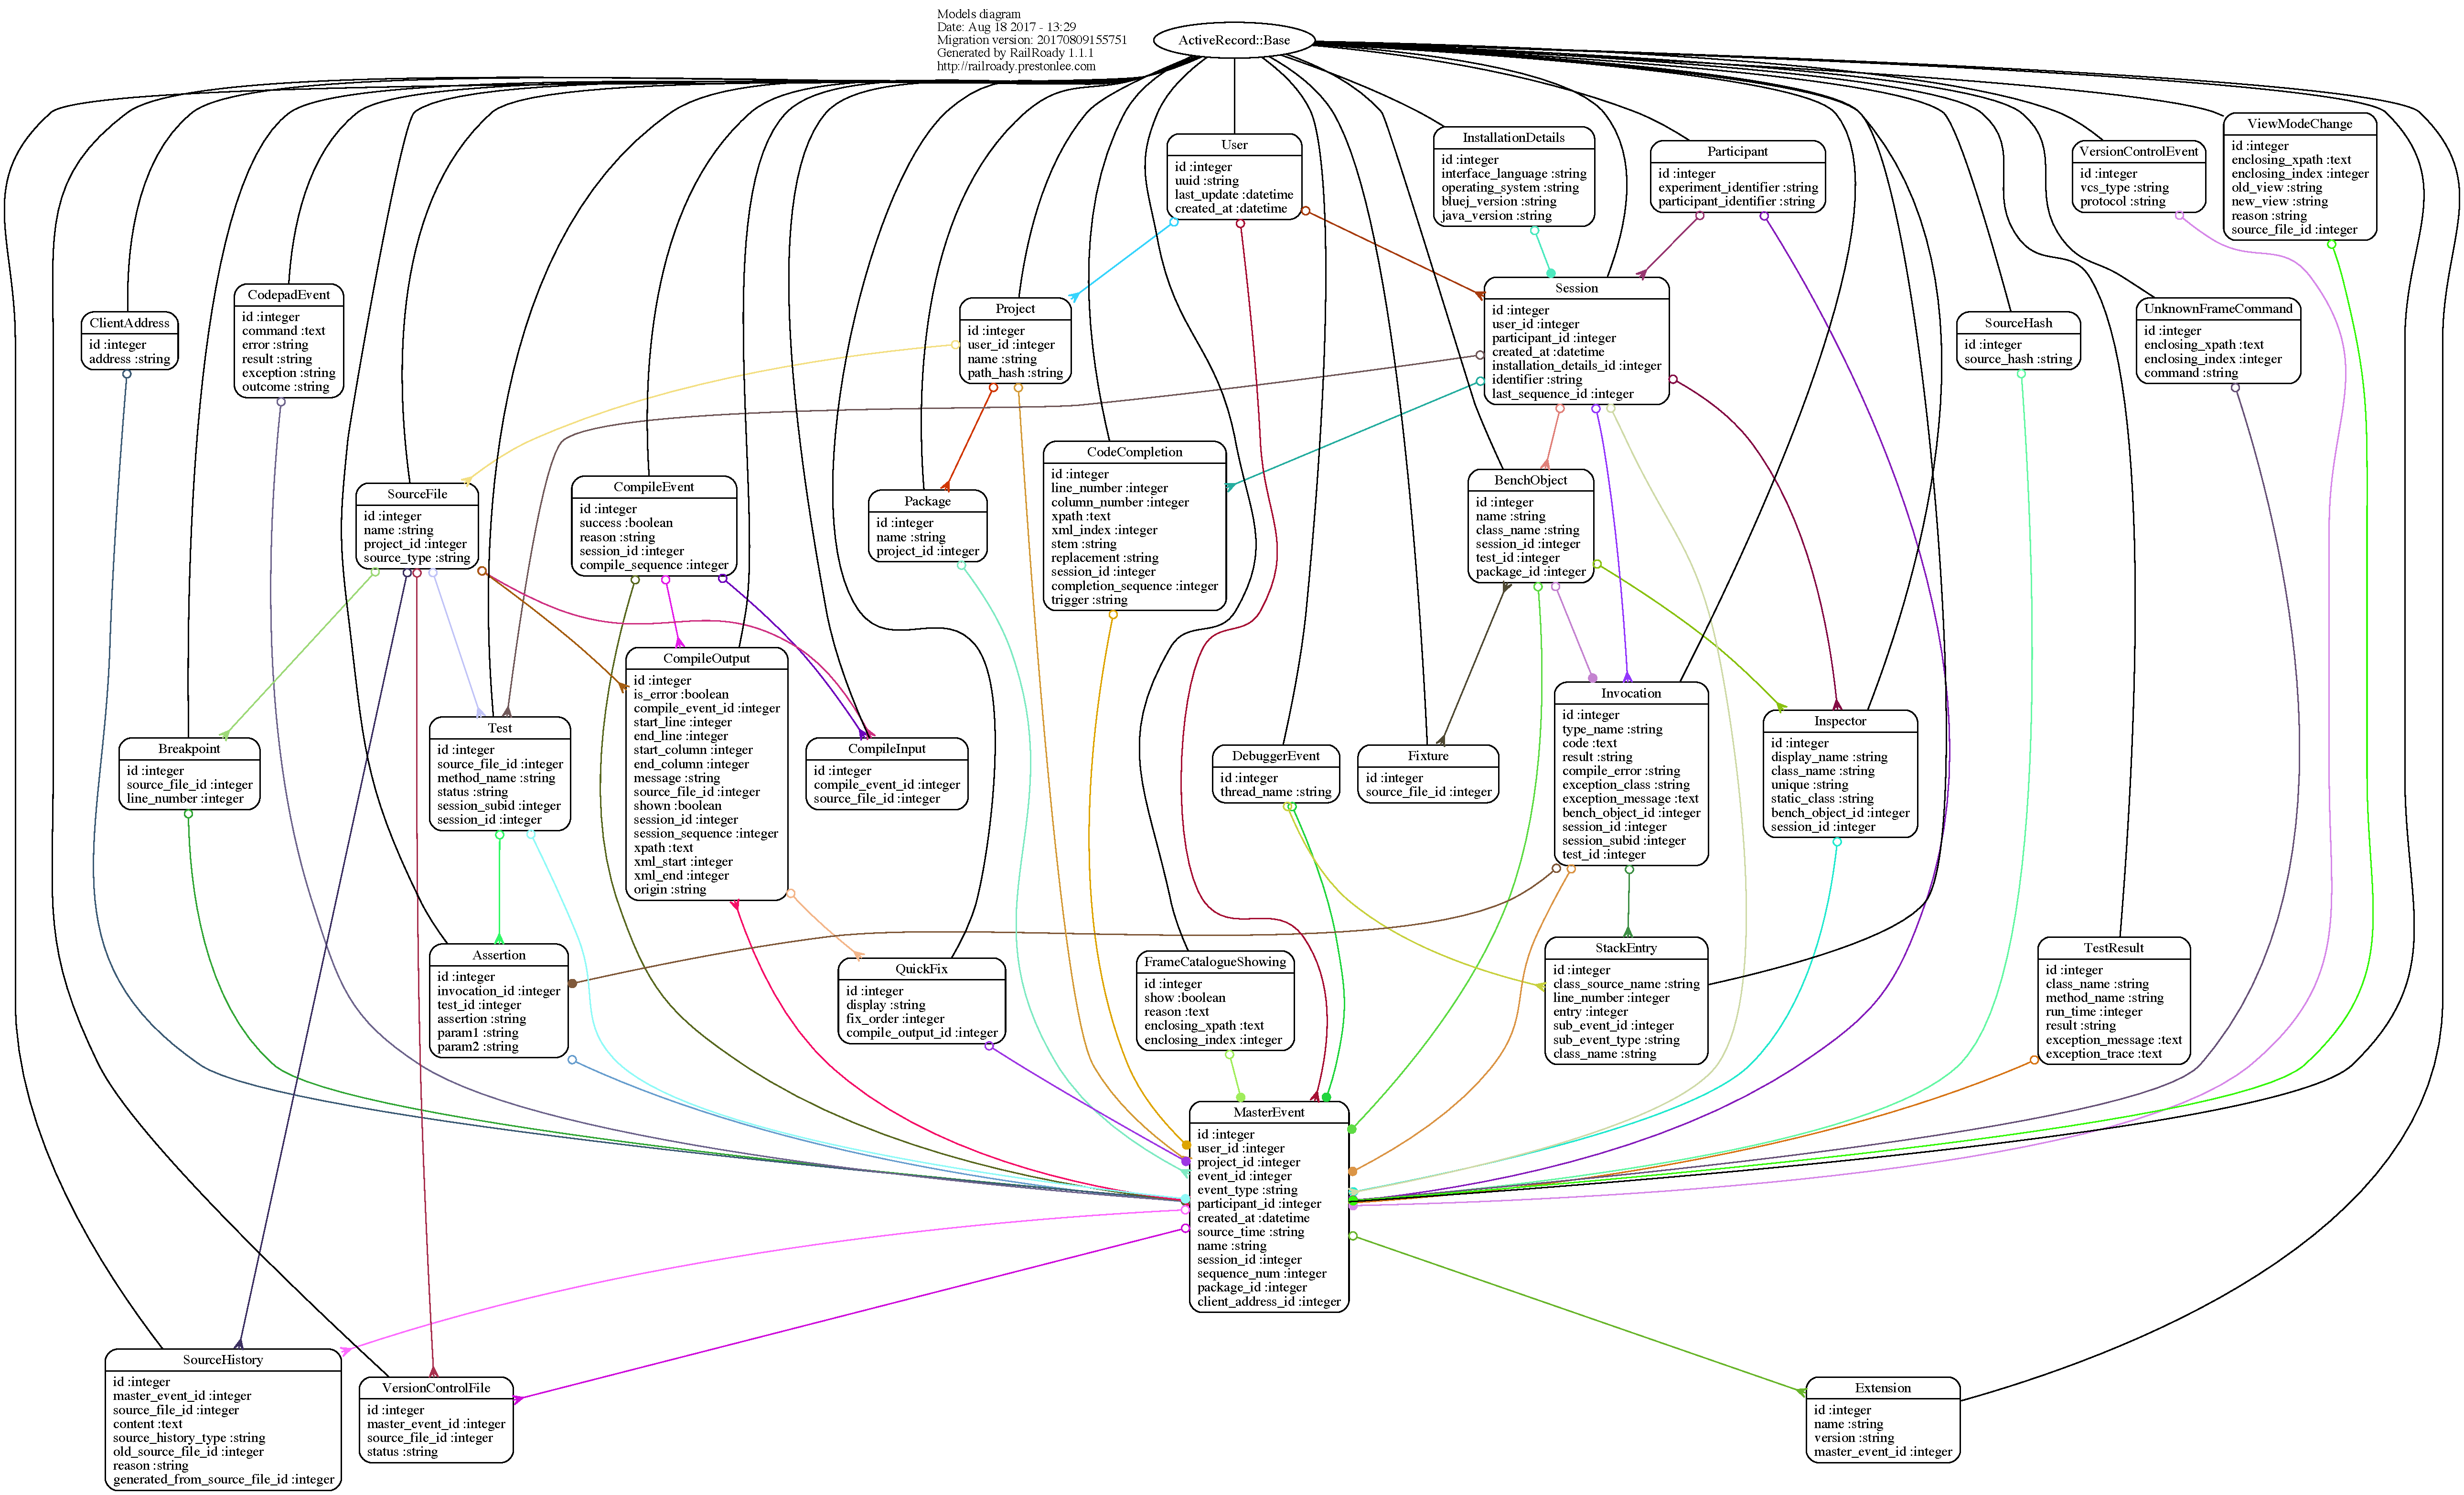
\includepdf[pages={1},landscape=true]{models.pdf}

\chapter{Analysing Blackbox Subsets}

Blackbox can be roughly divided into three parts:
\begin{enumerate}
\item Manual-Java: the events from BlueJ 3.x, which only featured Java as a source language, and where compilation was always manually triggered.
\item Auto-Java: the Java-related events from BlueJ 4.x.  The editing events are almost identical to BlueJ 3.x, but error-check compilations are performed in the background, which means compilation needs to be analysed differently.
\item Stride: the Stride-related events from BlueJ 4.x.  The editing events are similar to Java, and use the same tables, so need to be accounted for if you only want to analyse Java.  Compilation events also happen in the background, as for auto-Java.
\end{enumerate}

The following sections describe what to watch out for if you only want to analyse a particular subset of Blackbox data.

\section{Only Java}

The |source_type| column of the |source_files| table is either |"java"| or |"stride"|.  So if you only want Java files, you will need to perform a join with the |source_files| table (e.g. joining with |compile_outputs|) to filter on this column.

\section{Only Stride}

The |source_type| column of the |source_files| table is either |"java"| or |"stride"|.  So if you only want Stride files, you will need to perform a join with the |source_files| table (e.g. joining with |compile_outputs|) to filter on this column.

\section{Only user compiles}

The |compile_events| table has a |reason| column.  For BlueJ 3.x compiles, when compilation always happened by the user explicitly clicking compile, the |reason| column is NULL.  If you only want to analyse coding where the user sees no errors until they click the compile button, you can just look for |reason| being NULL.  You'll have a good four years of data and over 200 million compile events.

BlueJ 4.x uses the |compile_events| table for recording several different types of compilation.  One type is when the user clicks compile, just as in 3.x.  In this case, the |reason| column will be |"user"|.  However, if you bundle together 3.x explicit compilations and 4.x explicit compilations, you're combining two different things.  In BlueJ 4.x, we also compile whenever the user leaves a modified line of code (same rule as when we send edits to Blackbox), and crucially we show the errors from this background compilation.  So in 3.x when the user clicks compile, they will either get success, or will get presented the first error from the compilation, which won't have been displayed (unless from a prior explicit compilation).  In BlueJ 4.x, they will either get success, or will be taken to the first error, which will likely already be showing because the background compilation found it.  They will also already be able to see any other errors in the file.  So the user is likely to click compile in different circumstances in 3.x (Do I have any errors?) to 4.x (Either: jump me to the error, or I'm finished and see no errors so do the real compilation now).

Bottom line: if you choose to analyse 3.x and 4.x compiles together, make sure that
 this makes sense for your analysis.

\chapter{Locations}
\label{sec:locations}

For some research questions, you may be interested in the location of a given user.
If you want to go as far as individual institutions, you will need to get the users
to tag themselves explicitly -- see \myref{sec:participants}.  If you just want country
information, then you can access that without any additional effort.

There is a |geocodes| database with a |geocoded| table.  This table has four columns:
\begin{itemize}
\item |client_address_id| -- This should be matched with the |client_address_id| column
in the |master_events| table.
\item |country_code| -- A two letter code identifying the country.
\item |country_name| -- The name of the country.
\item |continent| -- The continent which the country is located in.
\end{itemize}

You will generally involve this |geocoded| table in an inner join with the |master_events| table when
you want to retrieve country information, or narrow your search to specific regions.  For example, the
following query counts the number of compile events in North America:

\begin{lstlisting}
select count(id)
  from master_events
    inner join geocoded.geocodes
      on master_events.client_address_id = geocodes.client_address_id
  where
    name = "compile" and continent = "North America"
\end{lstlisting}

This query shows the number of sessions by country:

\begin{lstlisting}
select geocodes.country_name, count(id) as sessions
  from master_events
    inner join geocoded.geocodes
      on master_events.client_address_id=geocodes.client_address_id
  where name="bluej_start"
  group by geocodes.country_code
  order by sessions desc; 
\end{lstlisting}

The locations are determined by looking up the client's IP address in the Geolite2 database created by Maxmind,
available at \url{http://dev.maxmind.com/geoip/geoip2/geolite2/}.  So it is vulnerable to any mistakes
in that database, or use of a proxy in another country.  But generally, it should be trustworthy.

Note also that the |client_address_id| is stored with each master event.  Each event sent to Blackbox is
a separate HTTP request, so it is possible for the requests in a session to come from different IPs (e.g. if the user's DSL
connection reconnects during their BlueJ session).  It is hard to conceive of many situations where a user
would have IPs from multiple countries during a session, so in general it seems sensible to assume the country
is stable per-session.  However, it is a little more likely that a user may send events from multiple countries
over the course of several months, so be more wary about assuming a one-to-one mapping between user and country.

\chapter{Data Access}
\label{sec:data_access}

The data collection project involves two machines, running Ubuntu.  Each
machine has two 6-core hyperthreaded 2.5Ghz Xeon processors, with 32GB of RAM,
and four 2TB drives set up in RAID 5 configuration to hold the database.

One machine, nicknamed black, is
responsible for collecting the data.  It solely runs the MySQL database, and
the Ruby on Rails server.  

The second machine, nicknamed white, has a live-cloned database (named |blackbox_production|) from the recording
machine.  White is the machine to which you will have an account, and be able
to log in and perform data analysis.  The intention is that this way, nothing
that anyone does while examining the database on white can affect the
recording on black.

\section{SSH Access}

The white machine can be accessed by SSHing to |white.kent.ac.uk| on the
standard port (22).  The machine runs Ubuntu.  If you need any software
installed, then we can install any standard Ubuntu packages for you (email
|blackbox-admin@bluej.org|).

\section{MySQL}
\label{sec:ssh-tunnel}

The white machine runs MySQL on the standard port (3306) on the localhost
interface.  If you want to access the database directly from your own machine,
you can use an SSH tunnel:

\begin{lstlisting}
ssh -L 3307:localhost:3306 ssh_username@white.kent.ac.uk
\end{lstlisting}

While that SSH session is open, you can access the database by running:

\begin{lstlisting}
mysql -h 127.0.0.1 -P 3307 -u username -p blackbox_production
\end{lstlisting}

You will have been given the MySQL details separately when you got an account on the machine.

\section{Feed}

To get familiarity with the data collection, we provide a mechanism to observe
a live feed of your own data.  The live feed is available, from the
white machine, on |http://localhost:3080/feed|.  It is probably easiest to
port-forward 3080 to your local machine using:

\begin{lstlisting}
ssh -L 3080:localhost:3080 ssh_username@white.kent.ac.uk
\end{lstlisting}

Then access |http://localhost:3080/feed| on your own machine.  You can find
your own UUID in your |bluej.properties| file -- look for the line
|blackbox.uuid=...|.  If you paste your UUID into the feed page and click the
button, it will refresh every five seconds until closed (be warned!) to show
you the data for that UUID.  Looking at this webpage while running BlueJ
should give a good feel for what is being recorded.

\section{Analysis Process}

We anticipate that researchers will do some of their analysis on the white
machine, and some on their own machine.  The advantage of using the white
machine is that it is high-powered, and has immediate access to all of the
data, without needing to copy the data across the Internet.  The disadvantage
is that it can be a bit restrictive to operate on a remote machine for all
analysis.  Researchers may therefore want to do a split, with some
pre-processing on the white machine, followed by more investigation on their
own machine.

\section{Data Snapshot}

When researchers publish their data, they will specify their data source.  It
is worth remembering that the Blackbox data is continually being added to, so
it is also necessary to specify which time period data was used from.  We
suggest choosing a cut-off date (e.g. the beginning date of the analysis) and
ensuring that only data up until that cut-off date is used, so that the source
of the data can be correctly specified as ``the Blackbox data repository was
used, up until 2013-03-31''.  You can use the date stamps in the
\tabref{master_events} to decide which data to use in your study.  (Bear in
mind that this may bisect some sessions -- make sure you do not process the
events in a session which fall outside your cut-off date).

\chapter{Data Use Policies}
\label{sec:data_use}

The data that we collect is not public.  This is part of our ethics approval
-- it is only visible to us, and selected researchers (i.e. those to whom we
give an account on the white machine).  

\section{Data Caching/Copying}

We realise that researchers will ultimately end up taking some data (probably
processed) on to their own machine, as a pragmatic step during the analysis.
We ask that you act responsibly, and make sure that the raw data is not made
public, and also that you take care to not let your account on the white
machine be compromised.  If you need multiple researchers at your institution
to have access, we would prefer giving them all accounts rather than
encouraging the practice of sharing accounts (and thus passwords).


\section{Data Use}

The data is intended for education research, and is anonymous.  We expect you
to not attempt to identify any students or data within the database, except
your own, and that of any participants in a study for which you have ethical
approval.  In particular, we forbid any use of the data for the purposes of
plagiarism detection (and similar) in students at your local institution.  The
participation of the users in the experiment is conditional on the data being
anonymous, and should not have any negative impacts for the participants.

\section{Sharing and Publication}

Researchers should not share the data with anyone -- any other researchers
wanting access should ask us for accounts.  Obviously, at some point,
researchers may want to publish their findings.  We expect that the data will
either be published in an aggregated form (which thus retains anonymity), and
that any individual case studies/vignettes will be manually anonymised, if
necessary.

\chapter{Blackbox Bugs and Interruptions}

\section{Known Interruptions}

From time to time, the Blackbox data recording may be interrupted, for routine maintenance or to deploy changes/fixes to the data recording mechanism.
Unless otherwise noted below, the effects are the same each time: all sessions that attempt to send data during the time that the server is unavailable will stop sending data.  So many sessions will simply end when the server is taken down, and recording will only be resumed for that user next time they start BlueJ.  Known outages of longer than 1 minute are listed below:

\begin{itemize}
\item 28 Jun 2013, approx 0722 to 0724 UTC (2 minutes), before master event 731142
\item 16 Sep 2013, approx 0942 to 0949 UTC (7 minutes), before master event 15537698
\item 17 Sep 2013, approx 1345 to 1351 UTC (6 minutes), before master event 15884081
\item 23 Sep 2013, approx 1338 to 1354 UTC (16 minutes), before master event 21192150
\item 31 Dec 2013.  There was a DNS issue surrounding the bluej.org domain name, which affected Blackbox.  For a few days (approx 31 December 2013 to 3rd January 2014 inclusive), the DNS problem prevented most users sending data to Blackbox.  It is hard to pinpoint how many and for how long, as we can't know if they were able to use the cached DNS value, or when the new DNS arrived on their nameservers.
\item 28 Jan 2015, approx 1543 to 1550 UTC (7 minutes), before master event 553795798
\item 12 Jan 2016, approx 1627 to 1649 UTC (22 minutes), service intermittent between master event 1040343453 and 1040346172 exclusive
\end{itemize}

\section{Known Client Issues}

Blackbox was added in version 3.1.0 (released June 2013).  All versions from 3.1.0 to 3.1.7 (released February 2016) had full support for Blackbox data recording.  BlueJ 4.0.0 (released March 2017) through 4.1.0 (released June 2017) did NOT have support for Blackbox; anyone using these versions would not send any data to Blackbox, although their opt-in/opt-out preference would be remembered.  Once they upgraded to BlueJ 4.1.1 (targeted for release August/September 2017) or later would once again start sending data to Blackbox.

\section{Known Recording Bugs/Changes}

These sections are roughly ordered by the date at which they were fixed.

\subsection{Project Name Length}

From the beginning of the project until 28 June 2013 (master event 731142), the project name field was 64 characters.  A small handful of projects exceeded this length and were thus not recorded.  The length of the field was extended to 255 characters.

\subsection{Renames}

From the beginning of the project until 16 September 2013 (master event 15537698), renames were not being handled properly by the server.  These were relatively rare: for the 30 days leading up to the fix, there were around five renames each day.  Details are noted in the section on renames (essentially, the |old_source_file_id| column was added to fix this; if this is NULL for a rename event, it's because it predates the fix.)

\subsection{Case Sensitivity}

From the beginning of the project until 23 September 2013 (master event 21192150), the database was using a case-insensitive comparison on all fields.  This affected the following features.

Objects on the object bench would be located via a case-insensitive search for their name.  This means that if the user had two objects on the object bench with names that differ only by case (e.g. ``Obj1'' and ''obj1''), further events like method invocations may have referenced the wrong object.  Although you cannot be certain when the wrong object is referenced, it is possible to find if a session/package had two objects whose names differed only by case (i.e. where the error \textit{could} have occurred).  As of 26 September 2013, shortly after the fix, of 80567 sessions that used the object bench, 464 had objects with names that differed only in case (0.6\% of all sessions).

Packages within a project would be found via a case-insensitive search for their name.  Thus, if the user had two packages in the same project that differed only by case (e.g. ``MyPKG'' and ``mypkg''), further events may have referenced the wrong package.  Note that this problem is irrelevant on Windows, as it has a case-insensitive file system that would not permit two packages which differ only by case.  Having said that, changes to the case of a package may not have been correctly recorded by the system.  Use of any packages other than the default is relatively rare: less than 3\% of projects have a non-default package at the time of writing (26 September 2013).

Source files within a project would be found via a case-insensitive search for their name.  Thus, if the user had two source files in the same project that differed only by case (e.g. ``FOO.java'' and ``Foo.java''), further events may have referenced the wrong source file until the start of a new session after the server was fixed.  Note again that this problem is not possible on Windows.

Changes in the case of a source file (e.g. if a user renames their class from "FOO" to "Foo", causing a rename of the file from "FOO.java" to "Foo.java") would not have been noticed by the server: the case of the filename would not be kept up to date on the server side.  This would also have upset the source hash generated for this project thereafter.  Around 2\% of source hashes during the period were affected by these problematic renames.

\subsection{Source Hashes}
\lstset{columns=flexible,language=SQL,basicstyle=\ttfamily\color{black},keywordstyle=\bfseries\ttfamily\color{blue}}

From the beginning of the project until 17 September 2013 (master event 15884081), source hashes were \textit{potentially} different for two projects with the same contents.  Specifically, the order in which the source files were fed into the hashing was arbitrary.  Thus, assuming no interference from the case sensitivity mentioned above, a project with one file would always have generated the same hash.  A project with two files would have generated one of two different hashes, a project with three files would have generated one of six different hashes and so on.  During the period affected, around half of all source hashes were potentially affected (hashing was done when the source files were not in alphabetical order).

There is now a table available, named |source_hash_fix|, in a supplementary database also named |source_hash_fix| (on the same machine, with access available to the relevant MySQL users) that contains a list of fixed hashes to cope with the problems of ordering.  The |source_hash_fix| table has two columns: |master_event_id| (integer) and |source_hash| (string).  Simply, |master_event_id| is the |id| from the |master_events| table of a |"package_opening"| event, and |source_hash| is the fixed source hash for that |"package_opening"| event.  Running this query (which looks long due to including all the prefixes) shows us how many hashes were broken:

\begin{lstlisting}
select (blackbox_production.source_hashes.source_hash
          = source_hash_fix.source_hash_fix.source_hash) as matches,
       count(*) as count
  from blackbox_production.master_events
    inner join (blackbox_production.source_hashes, source_hash_fix.source_hash_fix)
      on (blackbox_production.master_events.event_id =
                blackbox_production.source_hashes.id
          and blackbox_production.master_events.id =
                source_hash_fix.source_hash_fix.master_event_id)
  where blackbox_production.master_events.name="package_opening"
        and blackbox_production.master_events.id < 15884081 group by matches
\end{lstlisting}

The output is:

\begin{tabular}{cc}
matches & count \\
0 & 242457 \\
1 & 297968 \\
\end{tabular}

Which is to say, 242,457 hashes were broken -- slightly under half of them.  To give an example of how you might use this fixed hash table, here is some SQL code I had written before I realised that the hashes were broken.  It retrieves all known hashes for a given project name:

\begin{lstlisting}
select source_hash
  from source_hashes
    inner join (master_events, projects)
      on (master_events.project_id = projects.id
          and master_events.event_id = source_hashes.id)
  where master_events.name='package_opening' and projects.name = ?
\end{lstlisting}

Afterwards, the same code concatenates the results of two queries:

\begin{lstlisting}
select source_hash
  from source_hashes
    inner join (master_events, projects)
      on (master_events.project_id = projects.id
          and master_events.event_id = source_hashes.id)
  where master_events.id >= 15884081
        and master_events.name='package_opening'
        and projects.name = ?

select source_hash
  from source_hash_fix.source_hash_fix
    inner join (master_events, projects)
      on (master_events.project_id = projects.id
          and master_events.id = source_hash_fix.source_hash_fix.master_event_id)
  where master_events.id < 15884081
        and master_events.name='package_opening'
        and projects.name=?
\end{lstlisting}

\lstset{columns=flexible,language=SQL,basicstyle=\ttfamily}
\subsection{Missing Data}

From the beginning of the project until 17 September 2013 (master event 15884081), the server was running slowly enough that we believe some data was lost.  This would manifest as some sessions ending early (as if the internet connection to the server had been severed) -- all received data should still be internally consistent and complete over the duration of the session until it cut out.  We believe this affected roughly the period from 26th August to 17th September (increasingly so towards the end of the period).

We are using figure \ref{fig:data-loss} -- our guess is as good as yours as to exactly how long before the fix we were losing data.  The cap on server load looks to have been around 15,000 events and it looks like this was reached the week beginning 26 August.  So the period of lost data might be around 26 August to 21 September.  Note that we would expect that the ramp-up from 24 August would not necessarily be proportional to the number of sessions -- because term starts in September, users are likely to use BlueJ for longer periods.  For example, compare the ratio of events to sessions or users in July (when we were unlikely to have been losing data) to the latest data in September: it is clear that the ratio is not constant.

\begin{figure}
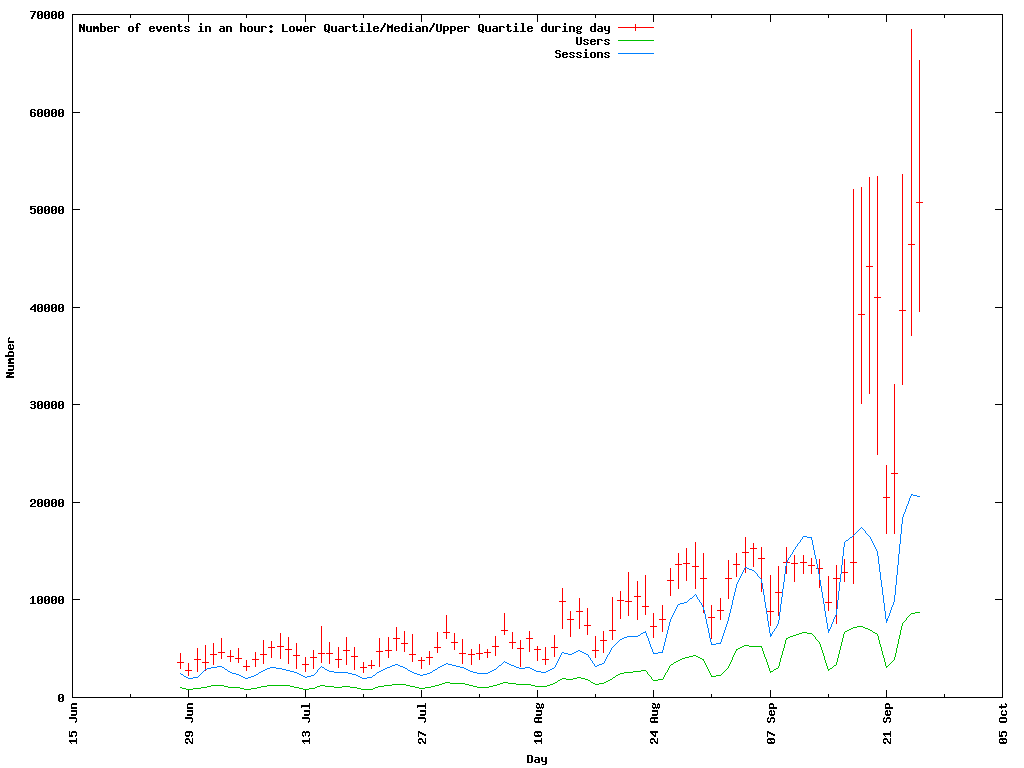
\includegraphics[width=\textwidth]{data-loss.png}
\label{fig:data-loss}
\caption{A graph up to 25 September 2013 illustrating the data loss until 17 September 2013.  The green line shows the number of users on each day, and the blue line shows the number of sessions on each day.  The weekly cycle is obvious.  You can see that the number of users and sessions did not increase after the date of the fix.  However, the amount of events received did increase markedly, as shown by the red bars.  To generate the red bars, we take the 24 hours of each day and work out the number of events in each hour.  Then we order the hours by their activity, and use the upper quartile (roughly, the 6th busiest hour), median (12th busiest) and lower quartile (18th busiest) to plot the bar which gives the spread of activity during the day.
}
\end{figure}

\subsection{Edits on Deleted Files}

There was a bug in BlueJ 3.1.0 and 3.1.1 where if you had edited a file immediately prior to its deletion, the events would be sent in the wrong order: the deletion event would be sent, followed by the pending edit.  This is relatively benign, but you must write your analysis software to cope: if you simply silently ignore all edits that occur on currently-deleted files, there should no negative consequence.  (It is unlikely you care what the edit was, given that the file was deleted immediately after, but if you do care you could just look for this situation and apply the edit before the deletion.)  This bug will be fixed in versions of BlueJ after 3.1.1.

\subsection{Renames and Bad Diffs}

There was a bug in BlueJ 3.1.0 and 3.1.1 that could occur surrounding renamed files and diffs.  There are two situations:

\begin{itemize}
\item If the destination file name had not existed before in this project and session, the next diff to the file would be against
a blank file, not against the contents of the file just before it was renamed.
\item If the destination file name had existed in this project and session (but had been deleted, or itself had been renamed),
the next diff would be against the old destination file (the deleted/renamed one) not the file that is the source of the rename.
\end{itemize}

In each case, it should be possible to work around this issue during the analysis stage by looking up the state of the destination file.
This problem will be fixed in versions of BlueJ after 3.1.1.

\chapter{Analysis Example: CodeView}
\label{sec:example_codeview}

We have created a simple proof-of-concept analysis tool (``CodeView'') to give a quick idea
of how analysis might work.  It appears to have a lot of code, but almost all
of it (in the |bluej.*| packages) is ripped from BlueJ -- code for displaying
the editor.

In the default package are five classes.  |IdName| is a simple data holder,
and |ListDialog| is a class to ask the user to pick an item from a list.  The
class |DatabaseInterface| has some Java code for interfacing with the
database.  It connects to localhost (assuming you are running the SSH tunnel
as described in section \ref{sec:ssh-tunnel}).  It demonstrates running a few
queries, given the UUID, to find a user's projects, and the files within a
chosen project.  For that file, the full history of the file is pulled.

The |SourceHistory| class uses the command-line |patch| application (available on all Unix-like systems) or any
to put the histories back together.  The |Viewer| class ties all this
together, and displays the source in a BlueJ editor window, and binds the
scroll wheel to moving backwards and forwards through the version history.

(Note: the sample has a slight irritation that the cursor is always moved to the end
of the file during scrolling, but the point is to demonstrate the database
queries and diffs and so on.)

\chapter{Additional Tools}
\label{sec:postprocess}

\textit{In time we will set up an area for this kind of information, but for
now, here are some details on tools and postprocessing tasks that we have
running on the ``white'' machine to aid analysis.}

\section{Extracted Compile Inputs}

The main likely area of analysis in the Blackbox project is looking at
the source code, especially at compilation time.  The way that the
source code is stored in the database (as a series of complete
snapshots, plus a stream of diffs) makes it a bit irritating to do the
source code analysis of compilations directly, as you have to
reconsitute the state of the source at each compilation.

To ease this process and save shared effort, we have a task that pulls
out the state of the source files each time they are compiled.  The
task runs overnight (GMT) in order to process the previous day.  In
the directory \texttt{/data/compile-inputs/} there is a series of files, one
per day, with all the compile inputs for that day.

The files named payload-YYYY-MM-DD are just one long stream of UTF8 strings;
to slice it up correctly you need to cross-reference
index-YYYY-MM-DD.  The index files are a long sequence of records,
with 32 bytes per record -- in order, they are:

\begin{itemize}
\item 64-bit integer for source file id.  (Corresponds to ``id'' column in
\tabref{source_files}.)
\item 64-bit integer for master event id for the compilation
event. (Corresponds to ``id'' column in \tabref{master_events}.)
\item 64-bit integer for the starting position within the payload
file. (Byte position in file, not character position in UTF8 string.)
\item 32-bit integer for the length within the payload file. (Again, byte
length, not character length.)
\item 32-bit integer that is 1 if the compile was successful, 0 if it was an
error.  (Copied from database for easy reference.)
\end{itemize}

All integers are big-endian.  If all you want to do is work
through all sources, you can just go through each index-payload pair
in turn, using the index records to slice the payload into different
inputs.  Otherwise, you can work forwards from the database: once you
find a compilation event you're interested in (say, one with a
particular error), look at the day on the master event.  Load the
index-payload for that day, and scan through to find the master event
id that you're looking for.  Obviously you can speed things up by
preloading all the indexes and forming a few hash maps or whatever.

\section{Tools}

In /tools/nccb/bin there are a couple of tools that you can use.

\begin{itemize}
\item |/tools/nccb/bin/print-source-hashes| takes a project name and then prints
a frequency table of source hashes for projects with that name.  You can use the
|--min-freq N| flag to set a minimum frequency (defaults to 5).
For example:

|/tools/nccb/bin/print-source-hashes shapes --min-freq 50|

\item |/tools/nccb/bin/print-compile-input| takes a path to the post-processed compile inputs
(|/data/compile-inputs| and then a numeric (denary) source file identifier and master event
identifier.  It then prints out the exact state of the source file at that compilation master
event.  For example:

|/tools/nccb/bin/print-compile-input /data/compile-inputs 1246 35238|

\item |/tools/nccb/bin/view-source-history| takes a source file identifier and then
allows you to scroll through the file, its source history and compile history.  For example:

|view-source-historyview-source-history 1234|

\end{itemize}
(Any other tools in /home/nccb/bin are irrelevant dependencies.)

\end{document}
